\documentclass{beamer}
\usepackage{polyglossia}
\usepackage{subfigure}
\usepackage{amsmath}
\usepackage{color, colortbl}

\usetheme{Boadilla}

\setdefaultlanguage{ukrainian}
\setotherlanguage{english}

\newfontfamily{\cyrillicfonttt}{Times New Roman}
\newfontfamily{\cyrillicfontsf}{Times New Roman}
\newfontfamily{\cyrillicfont}{Times New Roman}

\definecolor{LRed}{rgb}{1,.8,.8}

\title{Розробка засобів підбору та перевірки коректності УДК-шифрів наукових робіт}
\subtitle{121 Інженерія програмного забезпечення}
\author{студент групи ПЗ1911\\ Сафонов Данило}
\institute{Український державний університет науки і технологій\\
Факультет «Комп’ютерні технології і системи»\\
Кафедра «Комп’ютерні інформаційні технології»\\
}
\date{}

% Modify the footline template
\setbeamertemplate{footline}{%
  \begin{beamercolorbox}[wd=\paperwidth,ht=2.25ex,dp=1ex]{footlinecolor}
    \hspace*{1em} % Adjust the left margin if needed
    % Place your content here, e.g., frame numbers, navigation symbols, etc.
    \insertframenumber{} / \inserttotalframenumber % Example: Display frame numbers
    \hfill % Adjust the spacing between elements if needed
    \vspace*{0.5ex} % Adjust the vertical spacing if needed
  \end{beamercolorbox}
}

\begin{document}

\begin{frame}
	\titlepage
\end{frame}

\begin{frame}
\frametitle{Популярність УДК}

% тут рассказиваю про популярность (типо зачем вообще єто нужно)
УДК \textemdash~ Універсальна десяткова класифікація

\begin{itemize}
	\item \~{} 150,000 бібліотек та 130 країнах світу
	\item NEBIS (The Network of Libraries and Information Centers in Switzerland)
	  \textemdash 2.6 мільйонів записів
	\item COBIB.SI (Slovenian National Union Catalogue) \textemdash 3.5 мільйони записів
	\item Hungarian National Union Catalogue (MOKKA) \textemdash 2.9 мільйонів записів
	\item VINITI RAS database
	  (All-Russian Scientific and
		Technical Information Institute of Russian Academy of Science)
		\textemdash 28 мільйонів записів
	\item Meteorological \& Geoastrophysical Abstracts (MGA) \textemdash 600 журналів
	\item PORBASE (Portuguese National Bibliography) \textemdash 1.5 мільйони записів
\end{itemize}

\end{frame}

% тут рассказиваю про сложность (типо в чем профит)
% + сказать про то что із аналогов найдени только научние работи, т.е. реально інструментов нет в откритом доступе
\begin{frame}
\frametitle{Складнощі використання УДК}

\begin{itemize}
	\item 9 класів
	\item >60,000 підкласів
  \item 10 синтаксичних поширень
  \item 6 поєднувальних символів
\end{itemize}

\begin{center}
	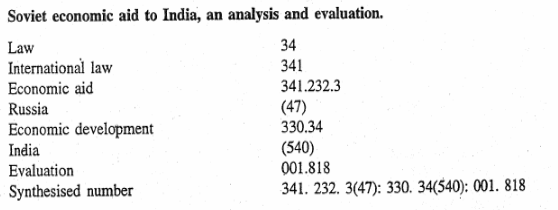
\includegraphics[width=9cm, angle=-0.5]{long_udc_example.png}	
\end{center}

\end{frame}

% Тут расскажу про то кто і как будет юзать
\begin{frame}
\frametitle{Use-case}

\begin{center}
	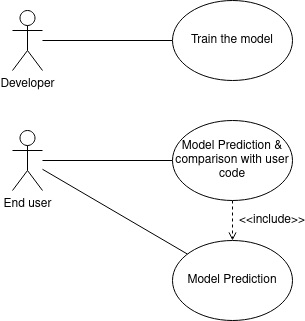
\includegraphics[width=6cm]{use-case.drawio.png}
\end{center}

\end{frame}

% tut +- toje samoe sho v ot4ete

\begin{frame}
\frametitle{Архітектура}
\begin{center}
	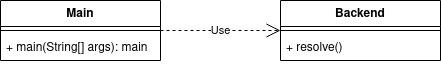
\includegraphics[height=1.5cm]{io_uml1.drawio.png}
\end{center}
\end{frame}

\begin{frame}
	\frametitle{Архітектура. Модуль користувацького інтерфейсу}
	\begin{center}
		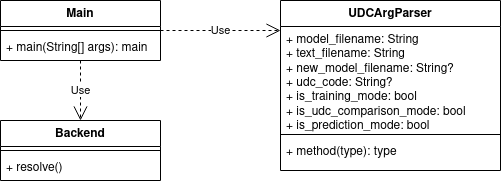
\includegraphics[height=3cm]{io_uml2.drawio.png}
	\end{center}
\end{frame}

\begin{frame}
	\frametitle{Архітектура. Режими роботи додатку}
	\begin{center}
		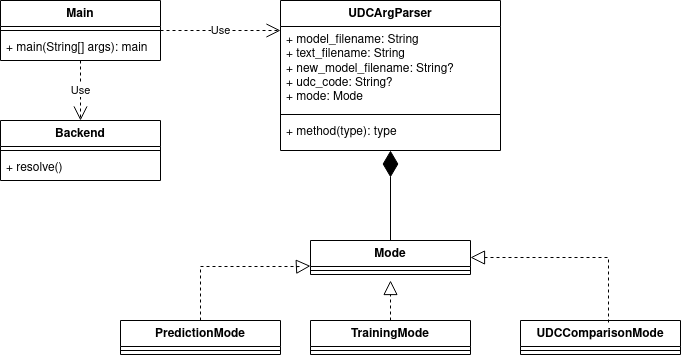
\includegraphics[height=5cm]{io_uml3.drawio.png}
	\end{center}
\end{frame}

\begin{frame}
	\frametitle{Архітектура. Режими роботи додатку. SRP}
	\begin{center}
		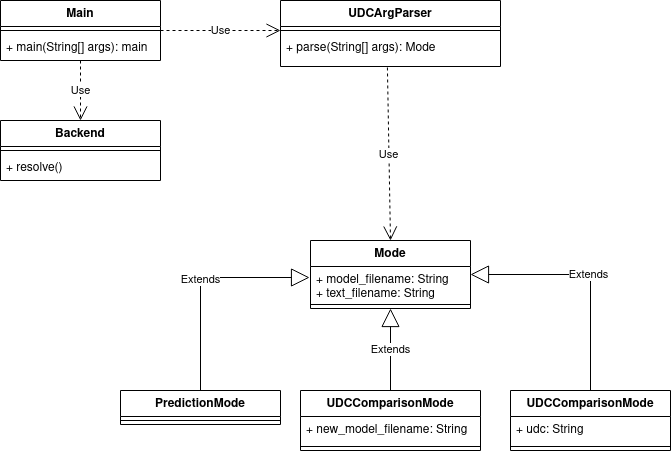
\includegraphics[height=6cm]{io_uml4.drawio.png}
	\end{center}
\end{frame}

\begin{frame}
	\frametitle{Архітектура. Абстракція типів вхідних даних}
	\begin{center}
		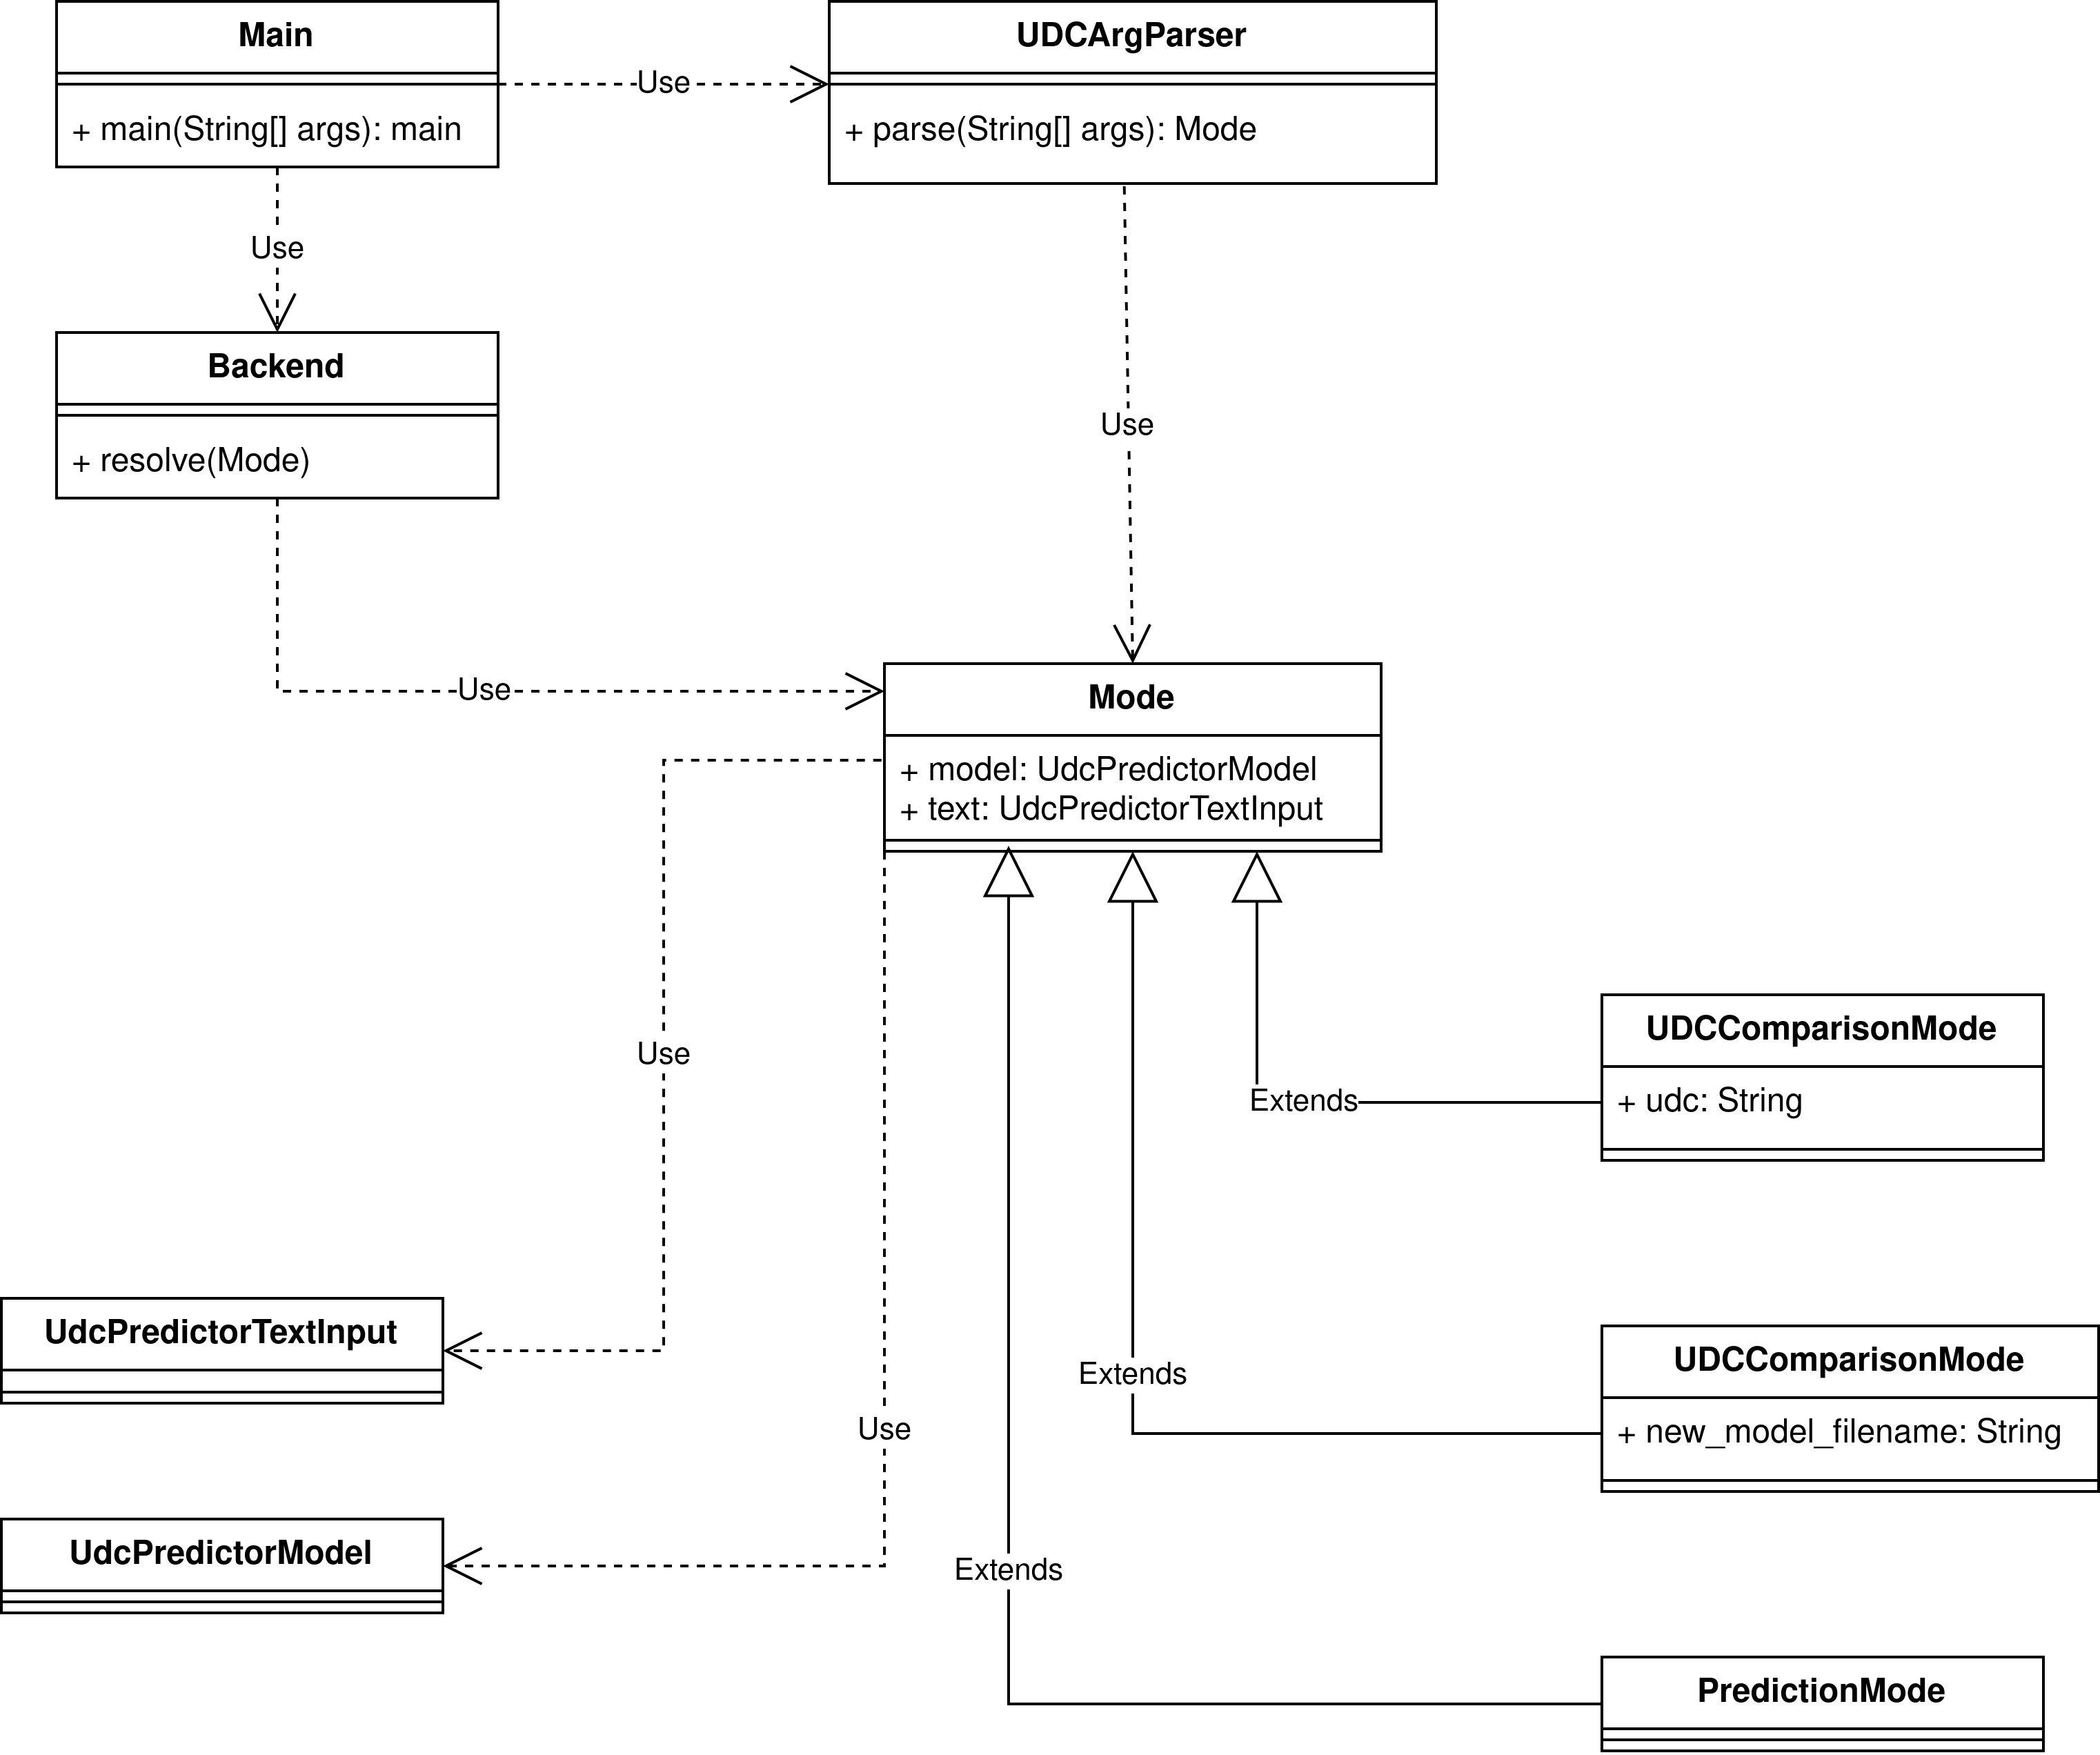
\includegraphics[height=7cm]{io_uml5.drawio.png}
	\end{center}
\end{frame}

\begin{frame}
	\frametitle{Фінальна архітектура}
	\begin{center}
		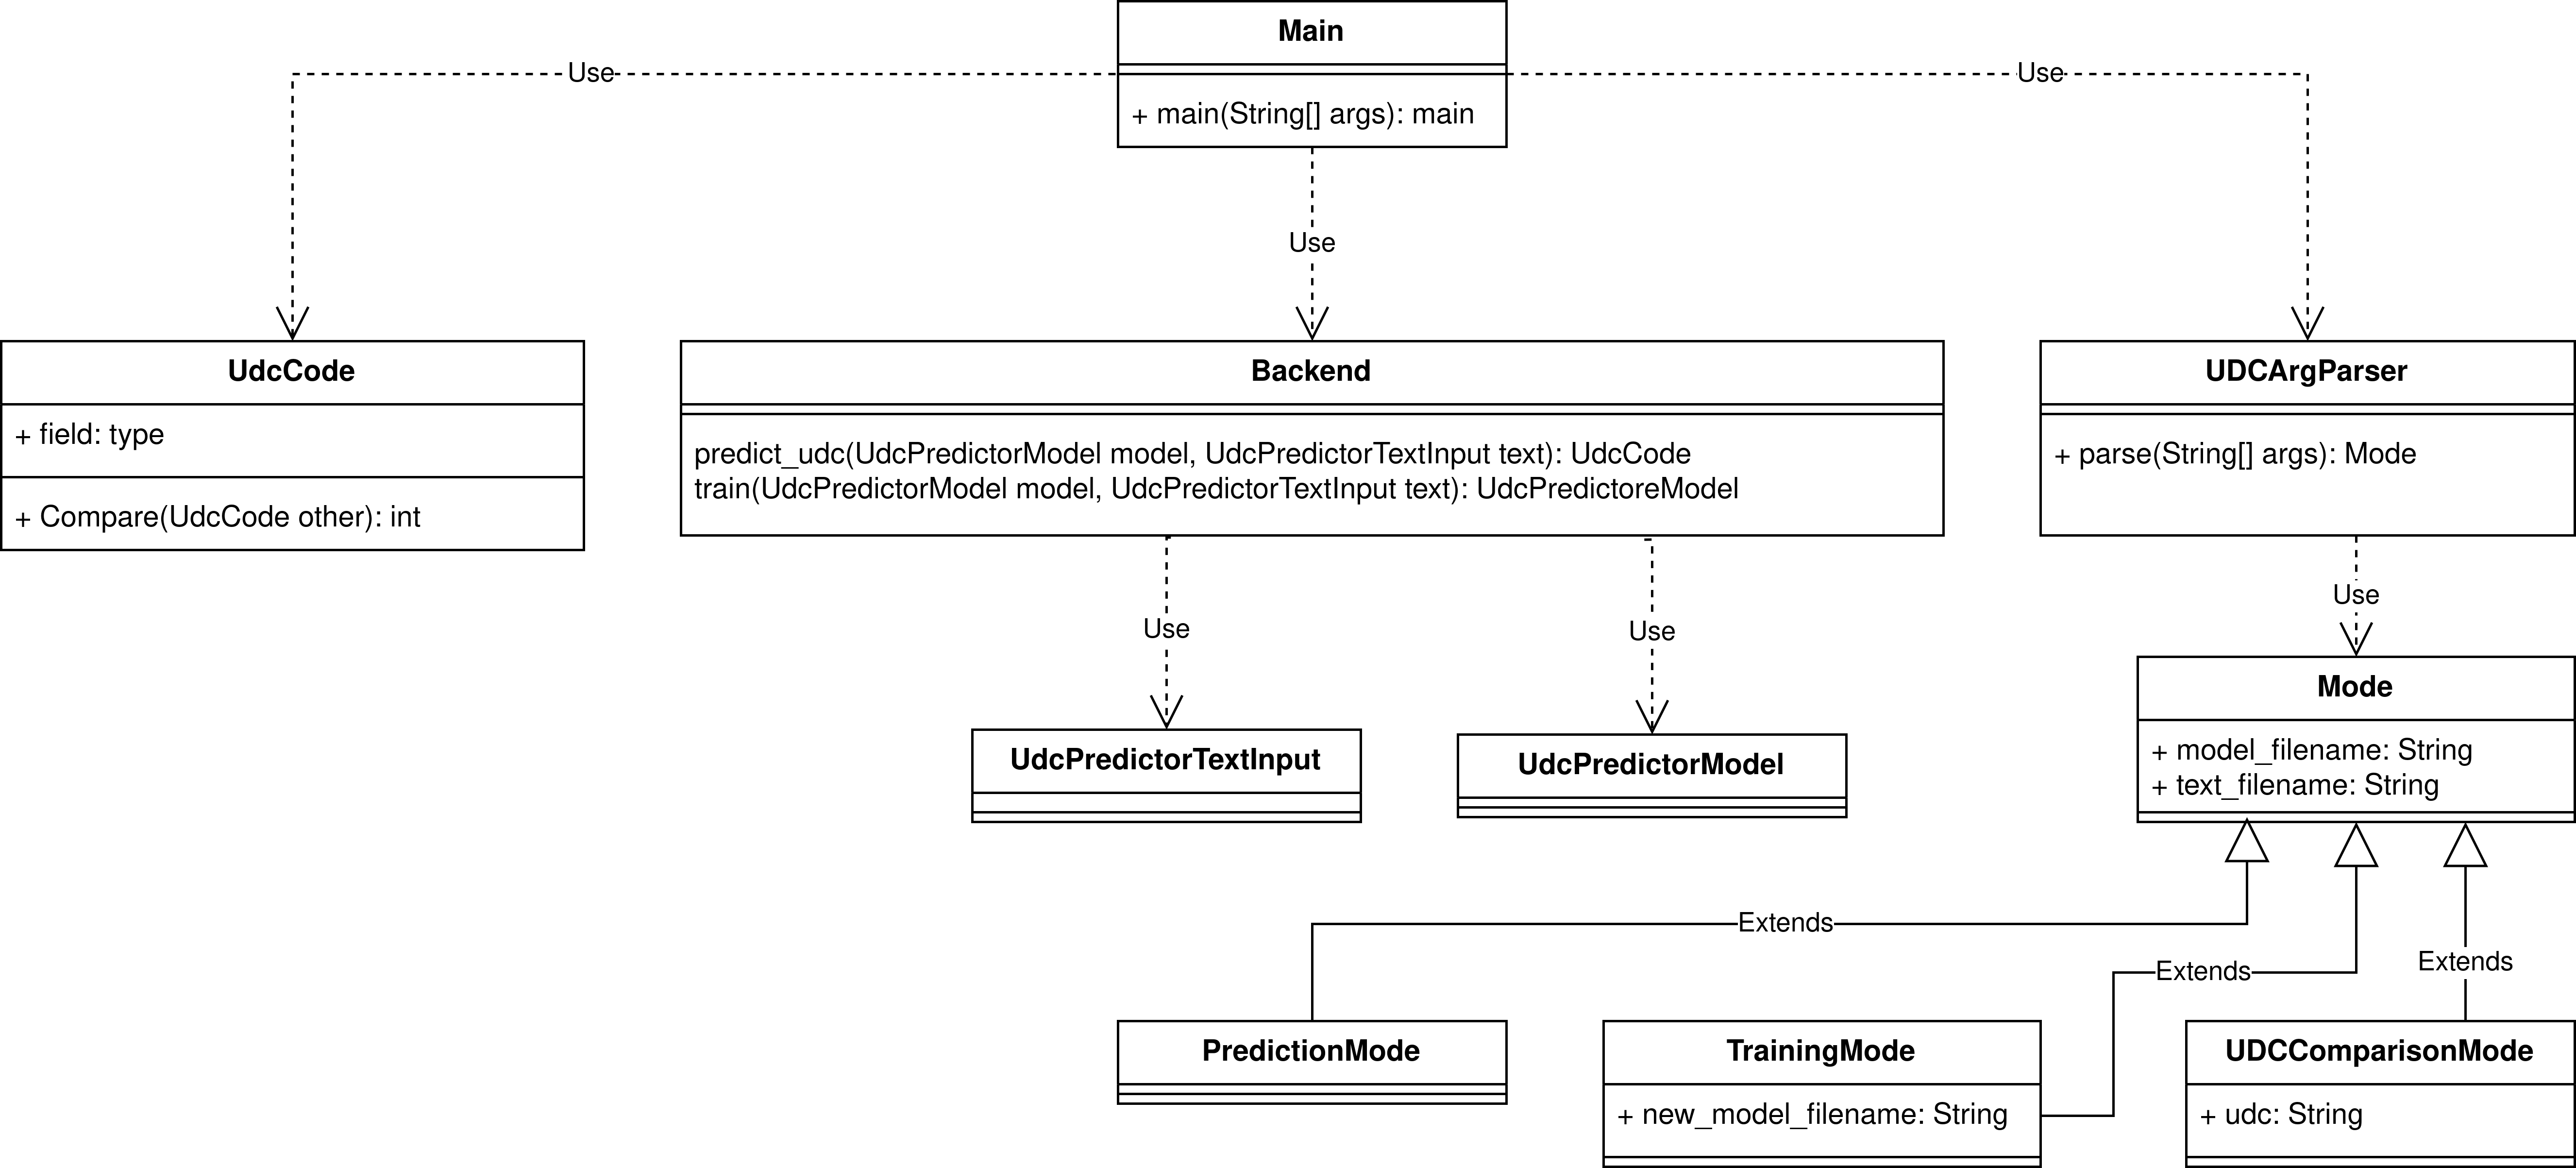
\includegraphics[height=5cm]{io_uml6.drawio.png}
	\end{center}
\end{frame}

% tut kratko poyasnu pochemu pituhon (populyarniy + podderzhka)
% spacy - kratko sravnit s ostalinimi varikami
\begin{frame}
	\frametitle{Засоби програмування}
	\begin{figure}
		\centering
		\subfigure{
\includegraphics[height=2.5cm]{python.png}}
		\subfigure{
\includegraphics[height=2.5cm]{spacy.png}}
	\end{figure}
\end{frame}

% rasskazivaem 4e toml
\begin{frame}
	\frametitle{Вибір формату серіалізації}
	\resizebox{\textwidth}{!}{%
		\begin{tabular}{|c|c|c|c|c|}
			\hline
			Формат   & Підтримка мов програмування & Читабельність & Структура даних & Стандартизація \\
			\hline
			CSV      & 9/10                        & 5/10          & 3/10            & 3/10 \\
			JSON     & 9/10                        & 5/10          & 6/10            & 9/10 \\
			Protobuf & 7/10                        & 1/10          & 8/10            & 9/10 \\
			\rowcolor{LRed}
			TOML     & 6/10                        & 9/10          & 9/10            & 9/10 \\
			XML      & 9/10                        & 5/10          & 9/10            & 10/10 \\
			YAML     & 6/10                        & 7/10          & 10/10           & 8/10 \\
			\hline
		\end{tabular}
	}
\end{frame}

\begin{frame}
\frametitle{Алгоритм витягування ключових слів з тексту}

\begin{equation}
	\begin{alignedat}{2}
	 keywords := ~&\{~ x \\
								&|~ n \in N &&~~,  ~ x = lowercase(n \setminus P) \\
								&           &&~~,  ~ x \cap S = \varnothing \\
								&           &&\land~ | text(x) | > 1 \\
								&           &&\land~ rank(x) <= c \\
								&\},
	\end{alignedat}
	\nonumber
\end{equation}

де n \textemdash~ іменникова група;
  
N \textemdash~ множина іменникових груп;

S \textemdash~ множина стоп слів;

w \textemdash~ слово в іменниковій групі;

P \textemdash~ множина знаків пунктуації;

rank \textemdash~ функція,
		яка повертає позицію елемента у множині за популярністю
		у порядку спадання;

c \textemdash~ кількість ключових слів, які потрібно обрати.
\end{frame}

% tut eshe vstavit 5 kopeek pro to kak model viglyadit
\begin{frame}
	\frametitle{Алгоритм перетворення ключових слів на класи УДК}
	\begin{equation}
    \begin{alignedat}{3}
      F := &\{~ (k,~ n(k,&&~ K)) ~|~ k \in K,~ &&K = K_p \cap K_u ~\} \\
      M':= &\{~ (k,~ f)  &&|~ (k, f)          &&~\forall ((k, f') \notin F
           \land   (k, f) \in M) \\
           &             &&                    &&\lor   ((k, f) \in F
           \land   (k, f') \notin M) \\
           &             &&,~ (k,~ f_f + f_m) &&~\forall (k, f_f) \in F \\
           &             &&                    &&\land   (k, f_m) \in M \\
           &\},
    \end{alignedat}
	\nonumber
\end{equation}
\end{frame}

\begin{frame}
	\frametitle{Порівняння списків класів УДК}
	\begin{equation}
    J(A, B) =  \frac{| A \cap B |}{ | A \cup B | }
    = \frac{| A \cap B | }{  |A| + |B| - | A \cap B | }
	\nonumber
\end{equation}
\end{frame}

\end{document}
